\section{Laborgeräte und Werkzeuge}
Im Umgang mit Laborgeräten ergeben sich mehrere Fehlerquellen, welche in der Auswertung von Versuchen relevant sein können. Zu dem sollte jeweils der Nutzen des jeweiligen Arbeitsmittels bekannt sein, um Messungenauigkeiten zu vermeiden.



\subsection{Allgemeiner Apparaturaufbau}
Egal ob Umkristallisieren, Filtrieren oder Destillieren:\\ \\
\begin{minipage}{0.45\textwidth}
	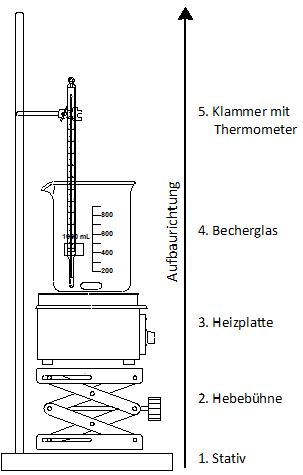
\includegraphics[width=0.8\textwidth]{img/Grundaufbau_Apparatur.png}
\end{minipage}
\begin{minipage}{0.55\textwidth}
		 Im Regelfall sollte eine Apparatur von "`unten nach oben"' aufgebaut werden. Die Arbeitsweise sichert den Halt und erleichter das strukturierte Auf- und Abbauen der Apparatur.
		 Ansonsten sollte man sich gerade in Angelegenheiten des Kühlens oder Heizens überlegen, wie die Höhe der Hebebühne einzustellen ist, um gegebenenfalls die Probe ohne Abbau der Messapparaturen zu erreichen.
\end{minipage}

\subsubsection{Schliffklemmen alias \textsc{Keck}-Clips}
Schliffklemmen bzw. \textsc{Keck}-Clips sichern die Verbindung zwischen Glasgeräten mit Normschliff. Diese Art von Schliffsicherung findet sich vorrangig im anorganischen und organischen Chemiepraktikum für den Aufbau größerer Apparaturen. Die Ausführung der Schliffklemmen ist verschiedenen Formen und Materialien zu finden. Eine häufig vertretende Form aus Kunststoff  sind die patentierten \textsc{Keck}-Clips.

\begin{figure}
	\begin{minipage}[b]{.45\textwidth} % [b] => Ausrichtung an \caption
		\centering
		\includegraphics[width=0.7\textwidth]{img/keck_clips}
		\caption{Skizze von \textsc{Keck}-Clips}
	\end{minipage}
	\hspace{.1\linewidth}% Abstand zwischen Bilder
	\begin{minipage}[b]{.45\textwidth} % [b] => Ausrichtung an \caption
		\centering
		\includegraphics[width=0.8\textwidth]{img/keck_clips_2}
		\caption{Beispielhafte Nutzung von \textsc{Keck}-Clips}
	\end{minipage}
\end{figure}
\FloatBarrier

\textit{Tipp:}\\
\vspace*{-5mm}

\fbox{\parbox{\linewidth}{
Um kleine oder leichte Apparaturteile, wie zum Beispiel Thermometer, zu montieren ist mit solchen Klemmen keine weitere Befestigung mehr nötig.}}

\subsubsection{Muffen}
Stativmuffen sind einer der häufigsten verwendeten Bauteil im apparativen Labor. Sie werden vorzugsweise für die Befestigung von zylindrischen Stativteilen, wie einer Stativklemme oder einem Stativring.
\begin{figure}[h!]
	\centering
	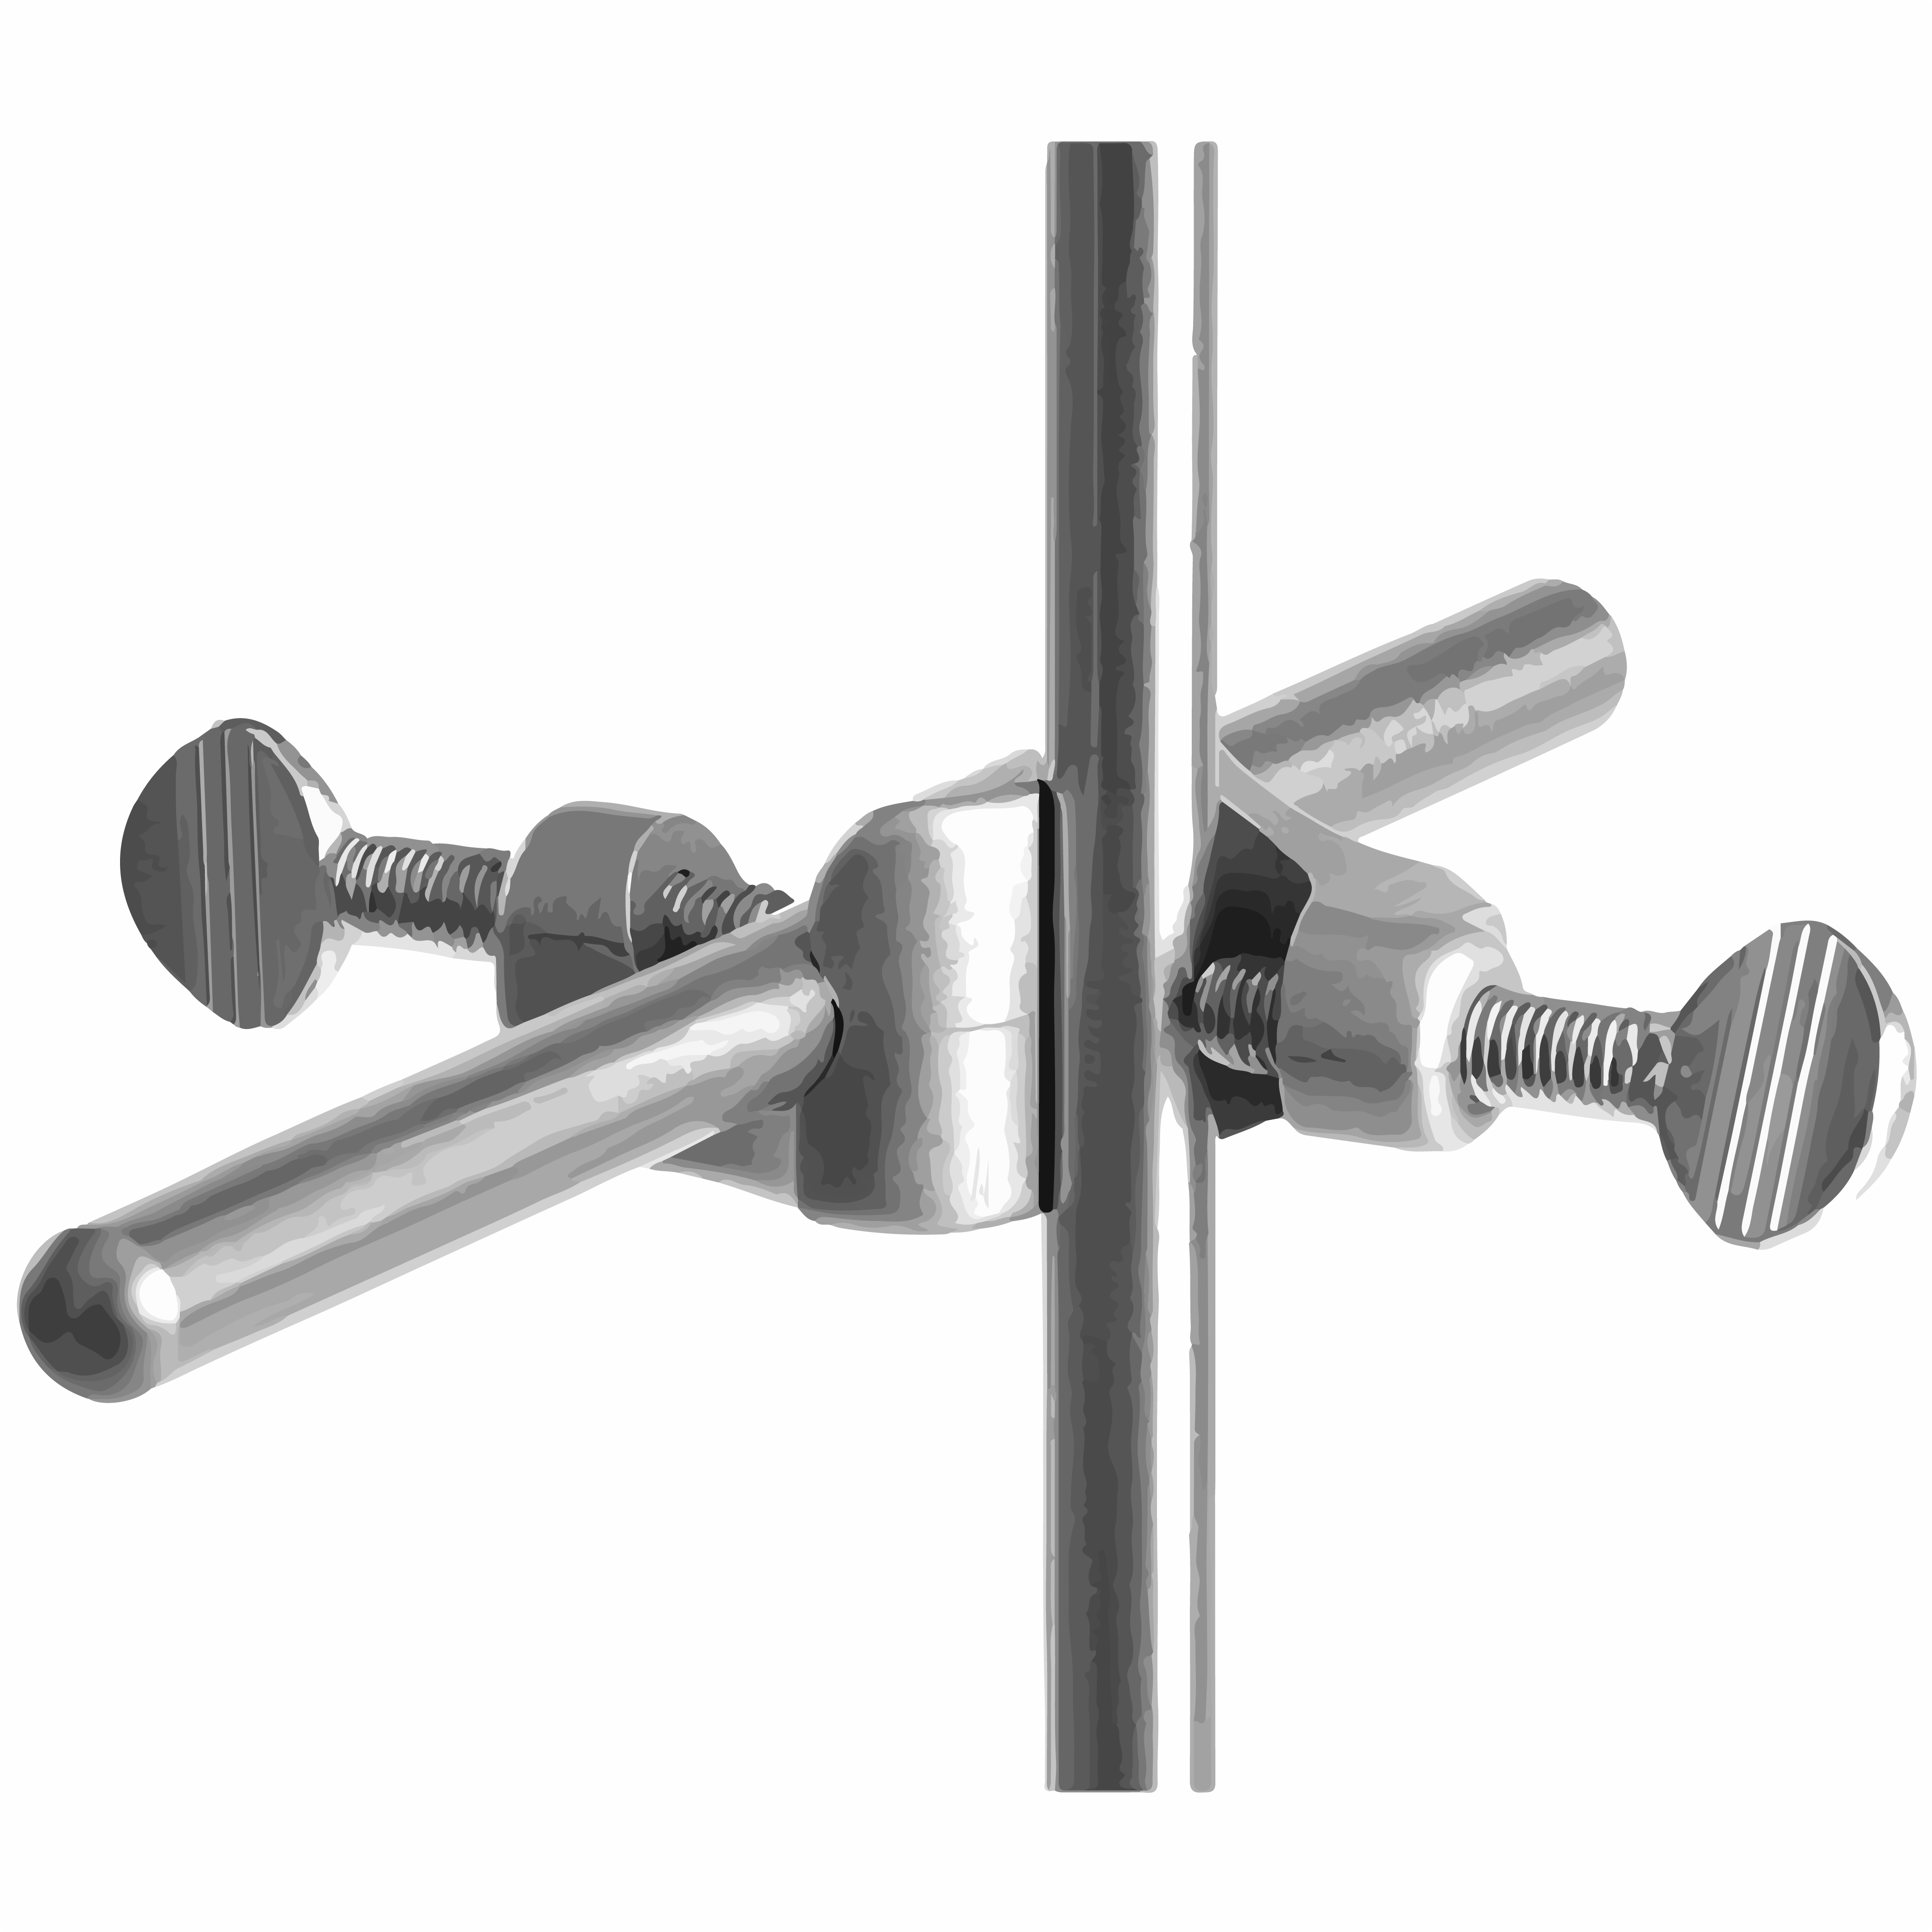
\includegraphics[width=0.5\textwidth]{img/muffe}
	\caption{Bild einer Stativmuffe}
	\label{fig:muffe}
\end{figure}
\FloatBarrier
%Ende

\subsubsection{(\textsc{Bunsen}-) Stative}
\textsc{Bunsen}-Stative bzw. Laborstative bestehen aus einer metallenen Grundplatte an welcher senkrecht eine Metallstange eingeschraubt ist. Sie dienen dazu verschiedene Versuchsaufbauten zu konstruieren indem an die die Stange mittels Muffen und Klemmen verschiedenste Hilfsmittel wie Gefäße, Büretten, Kochringe oder ähnliches in verschiedenen Höhen befestigt werden können.

\subsubsection{Korkringe}
Korkringe dienen zum Ablegen von Rundkolben, wenn diese nicht in ein Stativ eingespannt sind. Somit wird gesichert, dass Rundkolben aufgrund ihrer kugeligen Form nicht wegrollen.
\begin{figure}[h!]
	\centering
	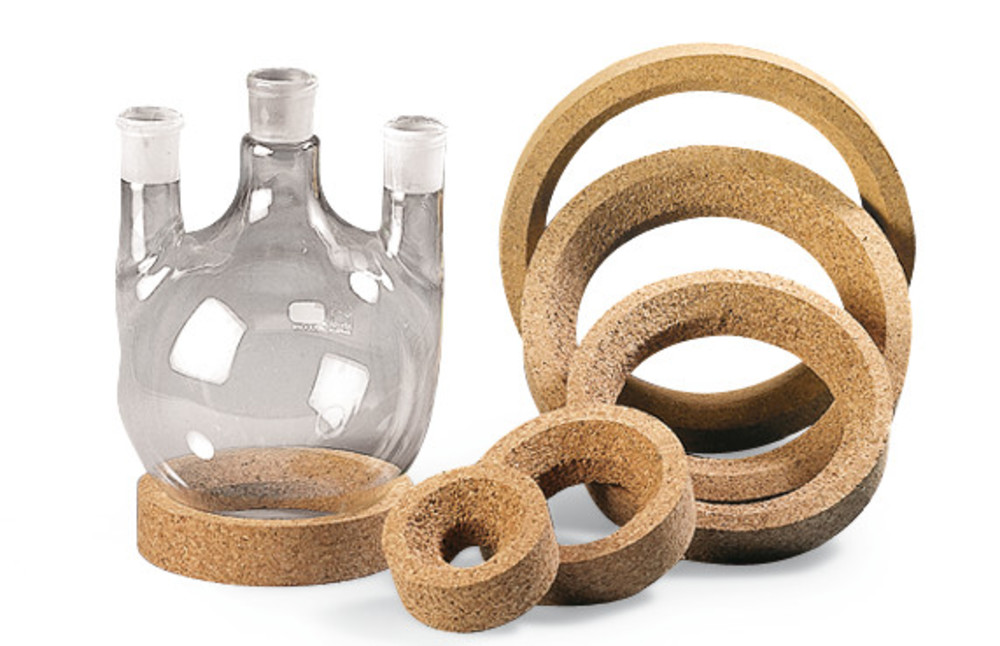
\includegraphics[width=0.45\textwidth]{img/korkring}
	\caption{Korkringe für Rundkolben}
	\label{fig:korkring}
\end{figure}
\FloatBarrier
%Ende

\subsubsection{Material der Glasgeräte}
Borosilikatglas Duran

\newpage

\subsection{Volumengefäße}
\subsubsection{Bechergläser}
Bechergläser sind zylindrische Becher, welche an der Oberseite einen gebogenen Rand, sowie eine Ausgussmöglichkeit haben. Sie werden für vielfältige Aufgaben, wie dem Erhitzen oder Zusammengießen von Flüssigkeiten. Es gibt sie in verschiedensten Ausführungen und Größen, welche meistens mit einem groben Maßstab versehen sind.\\
\vspace*{-5mm}

\textit{Hinweis:}\\
\vspace*{-5mm}

\fbox{\parbox{\linewidth}{
Messbecher sollten nicht genutzt werden um genaue Volumina zu messen. Besser eignen sich hierfür Messzylinder oder Maßkolben für das entsprechende Volumina.}}
\begin{figure}[h!]
	\centering
	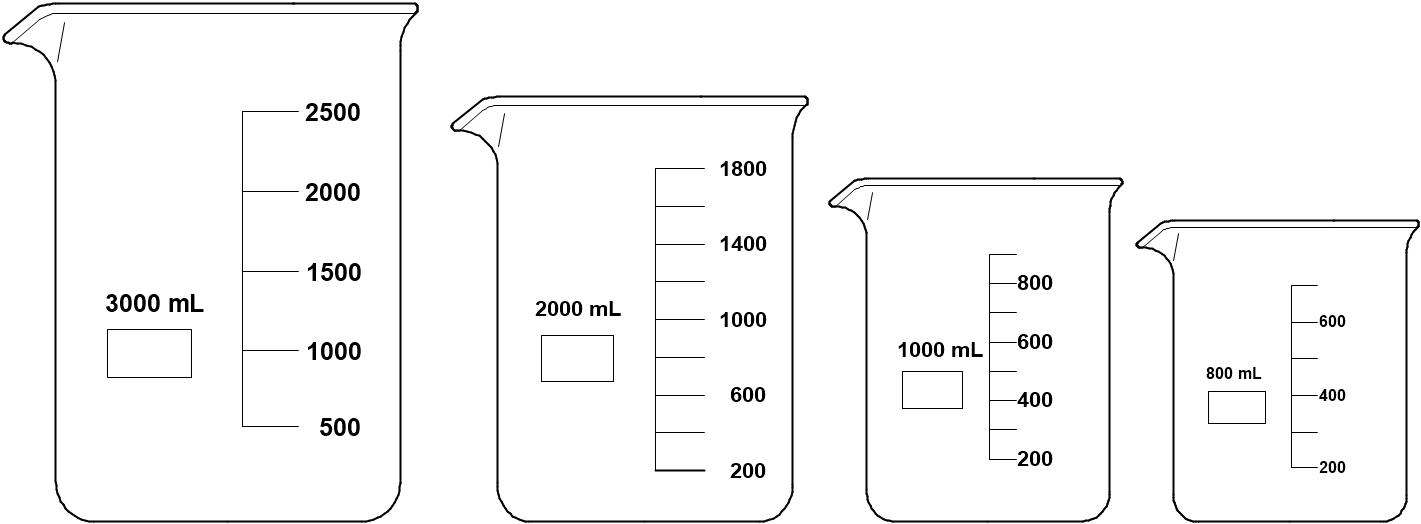
\includegraphics[width=0.45\textwidth]{img/becherglas}
	\caption{Bechergläser}
	\label{fig:becherglas}
\end{figure}
\FloatBarrier
%Ende
\vspace*{-10mm}

\subsubsection{Rundkolben}
Rundkolben werden ähnlich wie Bechergläser in den verschiedensten Größen und Ausführungen hergestellt. Viele der Kolben besitzen einen sogenannten Normschliff am Kolbenhals um beliebig und einfach gasdichte Apparaturen zusammenzustecken (mehr unter \hyperlink{Normschliff}{Normschliffe}). Des Weiteren können Rundkolben auch als Mehrhalskolben ausgeführt sein, um an den zusätzlichen Öffnungen zum Beispiel Kühler, Rührer, Messgeräte und/oder Zuläufe gleichzeitig anzubringen. Zusätzlich können Rundkolben, im Gegensatz zu Standkolben auch unter Vakuum genutzt werden, da die runde Form eine Implosion verhindert. Diese runde Form ermöglicht ebenfalls ein gleichmäßiges Erwärmen des Kolbeninhaltes.
\begin{figure}[h!]
	\centering
	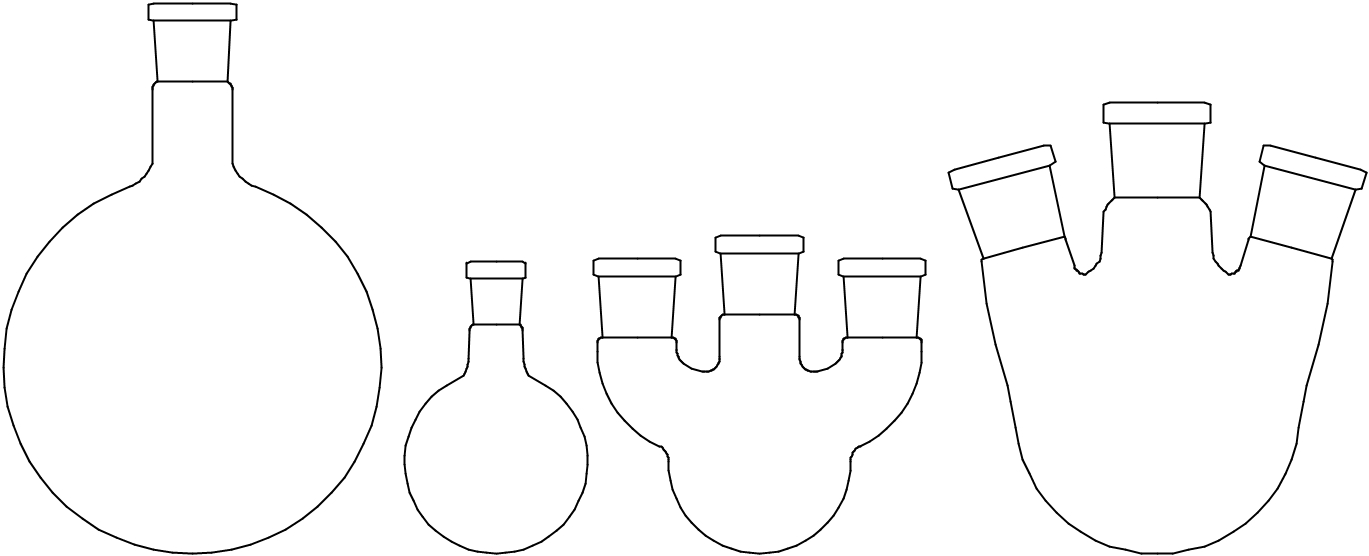
\includegraphics[width=0.45\textwidth]{img/rundkolben}
	\caption{Rund- und Mehrhalskolben}
	\label{fig:rundkolben}
\end{figure}
\FloatBarrier
%Ende

\subsubsection{Standkolben: Erlenmeyerkolben und Stehkolben}
Erlenmeyerkolben und Stehkolben unterscheiden sich im zum Becherglas vor allem im nach oben hin enger werdenden Hals. Dieser kann ebenfalls, wie bei den Rundkolben, je nach Anwendung mit einem Normschliff versehen sein. Gerade Erlenmeyerkolben werden aufgrund der Unterschiedlichen Ausführung des Kolbenhalses weiter in Enghals- und Weithalskolben klassifiziert. Der verjüngende Hals dieser Kolben minimiert maßgeblich die Gefahr, dass bei Zugabe von Substanzen, beim Schwenken, Rühren oder Sieden Flüssigkeiten unkontrolliert aus dem Kolben entweichen. 
Der Erlenmeyerkolben besticht dabei durch die Möglichkeit, die enthaltene Flüssigkeit gut zu Schwenken zu können, während der Stehkolben einen Rundkolben darstellt, welcher nicht wegrollen kann und eine druckstabiliere Bauweise glänzt.

\begin{figure}[h!]
	\centering
	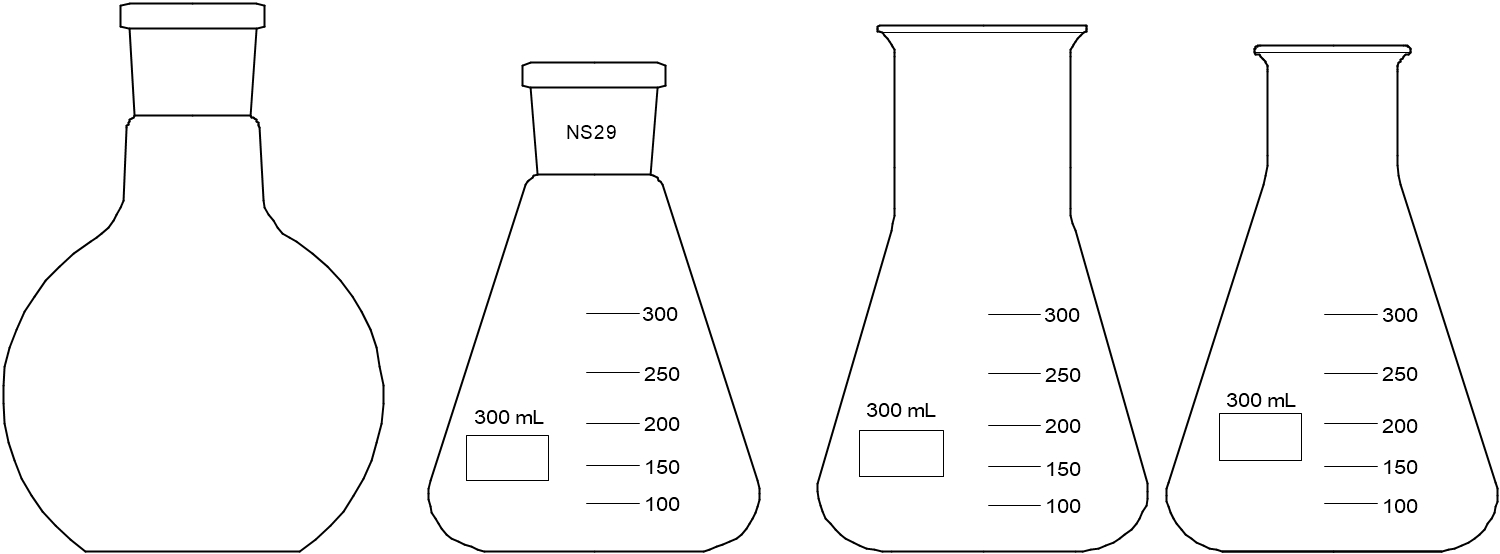
\includegraphics[width=0.65\textwidth]{img/standkolben}
	\caption{Standkolben}
	\label{fig:standkolben}
\end{figure}
\FloatBarrier
%Ende

\begin{table}[h!]
	\renewcommand*{\arraystretch}{1.2}
	\centering
	%\rowcolors{2}{white}{gray!25}
	\caption{Vergleich von Becherglas, Rund- und Standkolben}
	\label{tab:vergleich_becherglas}
	\resizebox{15cm}{!}{
		\begin{tabulary}{1.2\textwidth}{C|C|C|C|C}
			\hline
			 \diagbox{Eigenschaft:}{Kolben:}& \textbf{Becherglas} & \textbf{Rundkolben} &\textbf{Rundkolben}& \textbf{Erlenmeyer}\\
			\hline
			Magnetrührer & ja &ja & ja&ja\\
			hitzebeständig & ja &ja & ja&ja\\
			Mischung von Flüssigkeiten & ja &ja & ja&ja\\
			\hline
			selbststehend &ja&nein&ja&ja\\
			Normschliff &nein&ja&ja&ja\\
			gleichmäßiges Erwärmen &nein&ja&nein&nein\\
			vakuumfest &nein&ja&nein&nein\\
			\hline      
	\end{tabulary}}
\end{table}%
\FloatBarrier

\newpage

\subsubsection{Maßkolben bzw. Messkolben}
Maßkolben dienen hauptsächlich zum Ansetzen und Aufbewahren von Maßlösungen mit exakten Konzentrationen verwendet. Sie sind auf Einguss geeicht und zählen somit nicht unter die Kategorie Volumenmessgerät.\\
(Unter Maßlösungen versteht man Lösungen mit einer genau bestimmten Menge einer Substanz, welche über einen Urtiter bestimmt wird. Urtiter wiederum die gut wägbare Reinsubtanzen mit welchen sich der Gehalt von Maßlösungen bestimmen lässt.)

\begin{figure}[h!]
	\centering
	\includegraphics[width=0.15\textwidth]{img/Messkolben}
	\caption{Messkolben}
	\label{fig:messkolben}
\end{figure}
\FloatBarrier


\subsection{Messzylinder}


\subsubsection{Bürette}

%Küken von Tropftrichtern und brütten sind vorher zu testen! siehe Schlifffett

\subsection{Pipetten}
\subsubsection{Peleusball}
\subsubsection{Vollpipetten}
\subsubsection{Eppendorfpipetten}
\subsubsection{Hubkolbenpipette}

\subsection{Trichter}
\subsubsection{Flüssigkeitstrichter}
\subsubsection{Feststofftrichter}
\subsubsection{Tropftrichter}
\subsubsection{Scheidetrichter}

\subsection{Schläuche}
\subsubsection{Vakuumschläuche}
\subsubsection{Wasserschläuche}
\subsubsection{Oliven}

\subsection{Filter}
\subsubsection{Filterpapier}
\subsubsection{Fritte}
\subsubsection{Filternutsche}

\subsection{Waschflaschen}

\subsection{Rührer}
\subsubsection{Magnetrührwerk}
\subsubsection{Rührertypen}
\subsubsection{Rührermotor}

\subsection{Rückflusskühler}
\subsubsection{Dimrothkühler}
\subsubsection{Liebigkühler}

\subsection{Heizelemente}
\subsubsection{Wärmebad}
\subsubsection{Brenner}
\subsubsection{Heizpilz oder Heiznetz}
\subsubsection{Heizplatte}

\subsection{Pyknometer}

\subsubsection{Apparaturen zum Trocknen}
\subsubsection{Exsikkator}
\subsubsection{Trockenschrank}
\subsubsection{Muffelofen}

\subsection{Pumpen}
\subsubsection{Vakuumpumpe (Wasserstrahlpumpe)}
\subsubsection{Hubkolbenpumpe}
\subsubsection{Kreiselpumpe}

\subsection{Zusätzlich:}
\subsubsection{Beschriftung von Proben}
\subsection{Füllkörper}
\subsubsection{\hypertarget{Normschliff}{Schliffe} und Schlifffett}
\label{sec:normschliff}
\subsubsection{Ultraschallbad}
\subsubsection{Eismaschine}